\section{Korrelationsmatrizen sortiert nach der Bevölkerungsdichte}
\subsection{Landkreise}
In \autoref{fig:matrizes_pop_density_counties} finden sich die sechs Matrizen mit den Werten für die Korrelationen zwischen den Landkreisen. Die Zeilen und Spalten sind nach der Bevölkerungsdichte der Landkreise sortiert, eine vollständige Auflistung befindet sich im Anhang.

\todo{Anhang refernzieren}

\begin{figure}[H]
    \centering
    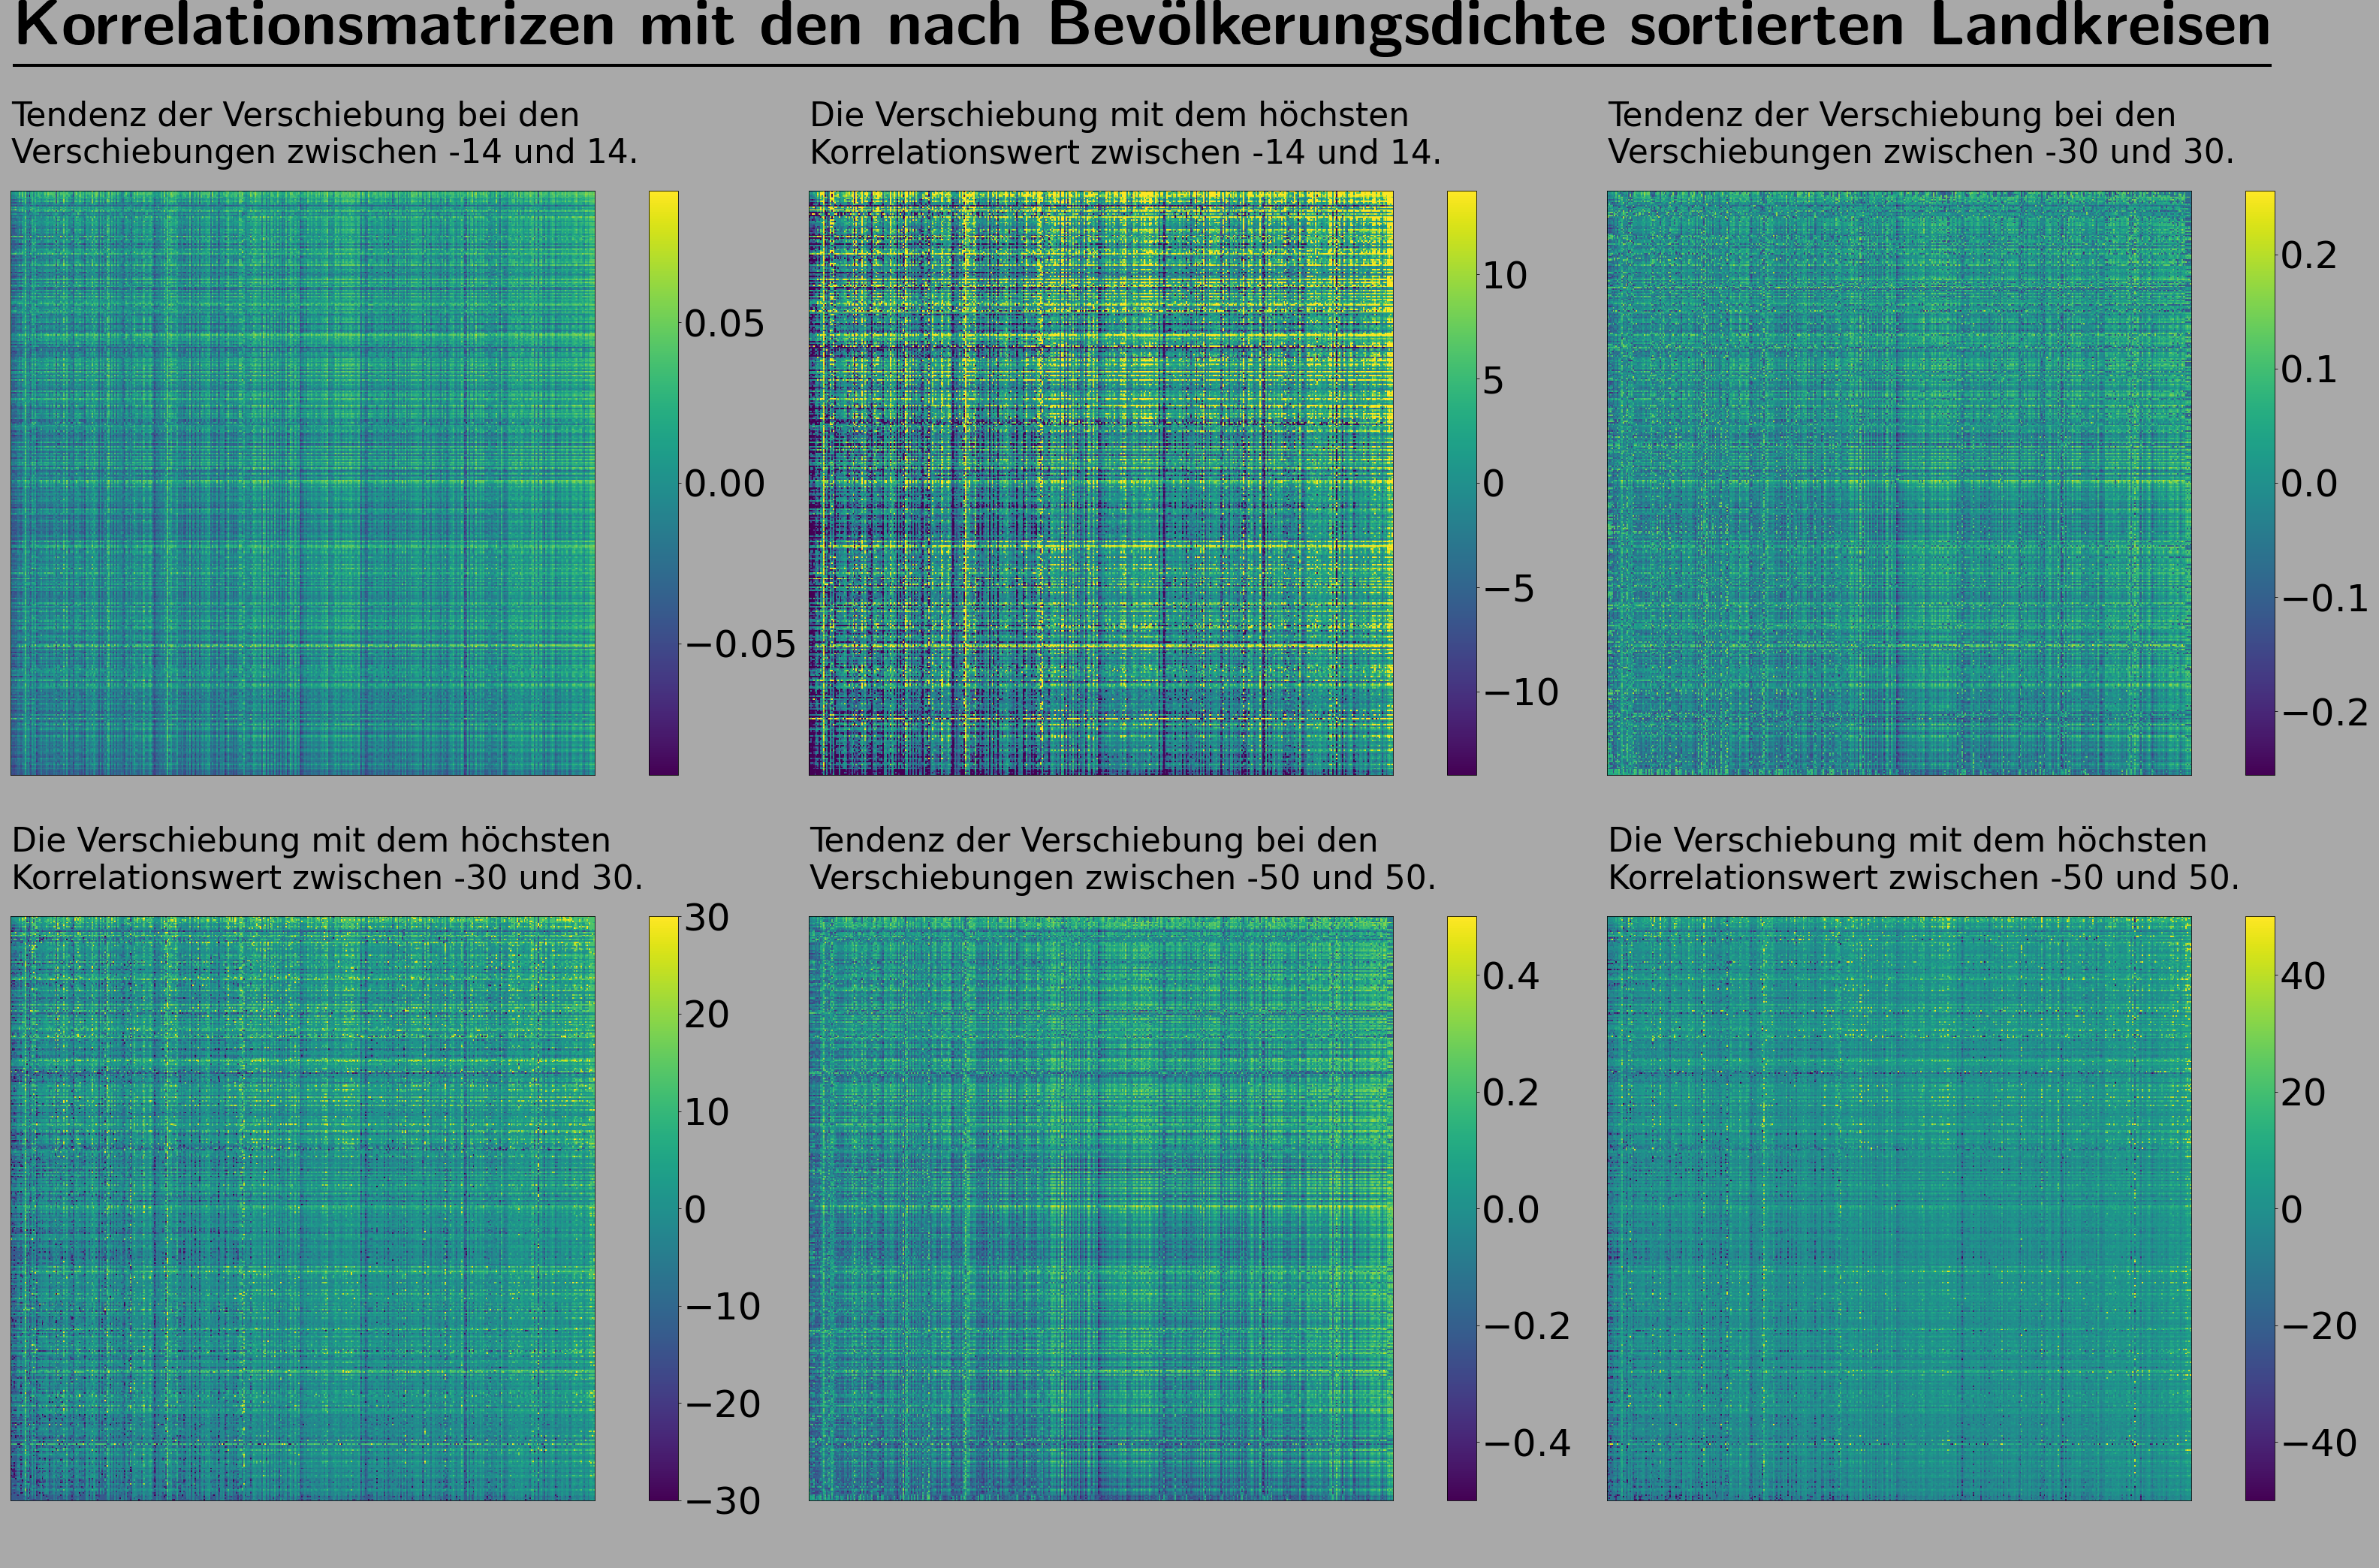
\includegraphics[width = 0.95\textwidth]{figures/Ergebnisse/matrizes_pop_density_counties.png}
    \caption{.}
    \label{fig:matrizes_pop_density_counties}
\end{figure}